\documentclass[sigconf,nonacm]{webmedia}
\usepackage[brazil]{babel}

\settopmatter{printacmref=false, printfolios=false}
\setevent{none}
\proceedingsDetails[Teoria dos Grafos]{Trabalho Prático de Teoria dos Grafos}{2026}{Salvador, Bahia}

\newcommand{\figura}[4]{%
  \begin{figure}[tbp]
    \centering
    \includegraphics[width=.94\linewidth]{imagens/#1.pdf}
    \caption{#2}
    \Description{#3}
    \label{#4}
  \end{figure}
}

\begin{document}

\title[Rede de coavaliação da Amazon]{Rede de coavaliação de produtos de videogame da Amazon}
\author{Jaedson Barbosa Macedo}
\affiliation{%
  \institution{Instituto de Computação, Universidade Federal da Bahia}
  \city{Salvador}
  \state{Bahia}
  \country{Brasil}}
\renewcommand{\shortauthors}{Macedo}

\begin{abstract}
Este trabalho analisa a rede de coavaliação de produtos da categoria
\emph{Video Games} do conjunto Amazon Reviews 2018, atribuída como
grafo G118. A rede é obtida pela projeção do grafo bipartido
usuário--produto: dois produtos são ligados quando ao menos dois
usuários avaliaram ambos, e a análise se concentra na maior
componente conexa, com 21\,284 vértices e 320\,742 arestas. Calculamos
as medidas estruturais da rede, implementamos os algoritmos clássicos
da disciplina, comparando complexidade teórica e tempo observado, e
investigamos as propriedades de pequeno mundo, lei de potência e
robustez. A rede é esparsa, tem caminho médio de 3,71 saltos e
clusterização elevada; contudo, essa clusterização é reproduzida por um
modelo nulo bipartido, o que indica um efeito da projeção, e não da
estrutura da rede. A distribuição de graus tem cauda pesada, mais bem
descrita por uma lognormal do que por uma lei de potência pura, e a
rede é robusta a falhas aleatórias e sofre degradação moderada sob
ataques direcionados: após remover 5\% dos vértices, a maior componente
retém 98,8\% dos remanescentes, contra 86,5\% no ataque por
intermediação, e quase toda a perda vem de vértices periféricos que
ficam isolados. Por fim, a rede reproduz a organização do mercado de
consoles: 55,2\% das arestas ligam produtos da mesma família de
console, contra 9,7\% esperados ao acaso, e os consoles concentram
ligações com outros consoles e acessórios.
\end{abstract}

\keywords{teoria dos grafos, redes complexas, coavaliação, projeção bipartida, pequeno mundo, robustez, homofilia}
\maketitle

\section{Introdução}

Uma avaliação na Amazon liga um usuário a um produto. Quando usuários
avaliam vários produtos, podemos usar as avaliações em comum para
construir uma rede em que os próprios produtos são os vértices. Neste
trabalho, usamos essa ideia para investigar como se conectam os itens da
categoria \emph{Video Games}, incluindo jogos, consoles e acessórios.

Organizamos a análise em três partes. A primeira descreve a estrutura
da rede. A segunda aplica algoritmos estudados na disciplina e compara
a complexidade teórica com os tempos medidos. A terceira investiga o
efeito de pequeno mundo, a distribuição dos graus, a robustez e a
relação entre as arestas e os rótulos de plataforma. Os resultados
estão nas Seções~\ref{sec:parte1} a~\ref{sec:parte3}, uma por parte,
e o código e os dados tratados estão disponíveis conforme a
Seção~\ref{sec:disponibilidade}.

\section{Determinação do grafo}
\label{sec:determinacao}

Seja \(S(M)\) a soma dos dígitos da matrícula \(M\) e
\(U(M)\) o número formado pelos dois últimos dígitos. O
índice é \(g=[S(M)(U(M)+1)]\bmod 129\). Para
\(M=224215943\), temos \(U(M)=43\) e
\[
  S(M)=2+2+4+2+1+5+9+4+3=32.
\]
Logo,
\[
  g=[32(43+1)]\bmod 129=1408\bmod 129=118.
\]
A regra usa 129 quando o resto é zero. O índice G118 corresponde a \emph{web-Amazon}
(\emph{Amazon reviews}) no catálogo da disciplina.

\paragraph{O grafo original.}
O \emph{web-Amazon} reúne 34\,686\,770 avaliações de 6\,643\,669
usuários sobre 2\,441\,053 produtos, de junho de 1995 a março de 2013,
distribuídas em arquivos por categoria, entre eles \emph{Video Games}
\cite{snapamazon}. Cada avaliação liga um usuário a um produto e traz
nota, texto e instante. Os dados formam, portanto, um grafo bipartido
usuário--produto, temporal e sem arestas diretas entre produtos.

\paragraph{Troca da base de dados.}
O grafo analisado não vem do arquivo listado na planilha da
disciplina. Os links de dados da página \emph{web-Amazon} do SNAP
remetem a um aviso que encaminha para a coleção mantida pela UCSD
\cite{snapamazon,acessosnap}. Dessa coleção usamos a edição
Amazon Review Data (2018), restrita à categoria \emph{Video Games}
\cite{amazon2018,ni2019}. A troca tem duas consequências: o período
passa a ser 1997--2018, e o recorte cobre uma única categoria. Por
isso, os tamanhos deste trabalho não se comparam aos da planilha.
Escolhemos \emph{Video Games} porque é um recorte viável que forma
uma rede interpretável de jogos, consoles e acessórios.

\section{Construção e tratamento da rede}

\subsection{Dos dados ao grafo bipartido}

Cada linha do CSV contém o identificador do produto (ASIN), o
identificador do usuário, a nota e o instante da avaliação. A base
bruta tem 2\,565\,349 linhas, 1\,540\,618 usuários e 71\,982
produtos, com registros de novembro de 1997 a outubro de 2018.
Usamos a avaliação como sinal de interação entre usuário e produto. A nota e o instante foram descartados para construir uma rede
estática, deixando de fora a satisfação do usuário e a evolução da
rede ao longo do tempo.

Sejam \(U\) o conjunto de usuários e \(P\) o de produtos.
A matriz de incidência \(B\in\{0,1\}^{|U|\times|P|}\) tem
\(B_{up}=1\) quando \(u\) avaliou \(p\). Assim, no grafo bipartido
\(\mathcal B=(U\cup P,E_B)\), cada aresta liga um usuário a um
produto. Denotamos por \(N(u)\) os produtos avaliados por \(u\) e
por \(N(p)\) os usuários que avaliaram \(p\). Seus tamanhos são
\(k_u\) e \(k_p\), respectivamente.

\subsection{Projeção por coavaliação}

Projetamos \(\mathcal B\) sobre \(P\). Para produtos distintos
\(p\) e \(q\), a aresta \(\{p,q\}\) existe se o peso abaixo é
positivo:
\[
  w(p,q)=|N(p)\cap N(q)|=(B^{\mathsf T}B)_{pq}.
\]
Cada usuário avalia um conjunto \(N(u)\), que gera um clique na
projeção. Quando outro usuário gera o mesmo par, somamos um ao peso.
Por exemplo, se \(a\) avalia \(\{1,2,3\}\), \(b\) avalia
\(\{2,3\}\) e \(c\) avalia \(\{3,4\}\), obtemos as arestas
\(\{1,2\}\), \(\{1,3\}\), \(\{2,3\}\) e \(\{3,4\}\).
Apenas \(\{2,3\}\) tem peso dois. O grau projetado de um produto
é limitado por \(\sum_{u\in N(p)}(k_u-1)\), pois dois avaliadores
podem gerar vizinhos repetidos. Isso ajuda a entender como produtos
populares se tornam vértices muito conectados.

\subsection{Tratamento dos dados}

Aplicamos os tratamentos abaixo uma vez e na ordem apresentada.

\begin{enumerate}
  \item \textbf{T1 -- Deduplicação.} Mantivemos uma ocorrência de
  cada par usuário--produto para que o mesmo usuário contribua uma
  única vez para cada par projetado.
  \item \textbf{T2 -- Limite por usuário.} Excluímos usuários com
  mais de 50 produtos avaliados. Cada usuário produz
  \(\binom{k_u}{2}\) pares, o que dá peso desproporcional a
  perfis com muitos itens e aumenta o custo da projeção.
  \item \textbf{T3 -- Mínimo por produto.} Após T2, mantivemos produtos
  com pelo menos cinco avaliadores. Usuários que ficaram com só
  um produto continuam no bipartido e geram zero pares.
  \item \textbf{T4 -- Projeção.} Construímos as arestas da parte
  triangular superior de \(B^{\mathsf T}B\), excluindo a diagonal.
  O resultado é um grafo simples, não direcionado e ponderado.
  \item \textbf{T5 -- Poda.} Mantivemos as arestas com \(w\geq2\),
  de modo que cada ligação resulte de pelo menos dois usuários
  distintos. Chamamos o grafo filtrado de \emph{backbone}.
  \item \textbf{T6 -- Maior componente.} Usamos BFS para contar as
  componentes do \emph{backbone}, incluindo os produtos isolados
  que passaram por T3. Extraímos a maior componente conexa (LCC)
  para as medidas que exigem conectividade.
  \item \textbf{T7 -- Custo de uma aresta.} Para caminhos mínimos
  ponderados e árvores geradoras, usamos \(d(p,q)=1/w(p,q)\).
  Mais avaliadores em comum reduzem esse custo.
  As medidas topológicas de distância usam número de saltos.
\end{enumerate}

\begin{table}[tbp]
\centering
\caption{Funil de preparação dos dados. Em T4 e T5, a coluna de produtos conta apenas os incidentes a uma aresta.}
\label{tab:funil}
\small
\setlength{\tabcolsep}{3.5pt}
\begin{tabular}{@{}lrrr@{}}
\toprule
Etapa & Usuários & Produtos & Linhas/arestas \\
\midrule
Bruto           & 1\,540\,618 & 71\,982 & 2\,565\,349 \\
T1 Deduplicação & 1\,540\,618 & 71\,982 & 2\,489\,395 \\
T2 Limite       & 1\,540\,162 & 71\,363 & 2\,449\,047 \\
T3 Mínimo       & 1\,508\,526 & 36\,626 & 2\,382\,072 \\
T4 Projeção     & --         & 36\,205 & 2\,509\,461 \\
T5 Poda         & --         & 21\,949 & 321\,127 \\
T6 LCC          & --         & 21\,284 & 320\,742 \\
\bottomrule
\end{tabular}
\end{table}

A Tabela~\ref{tab:funil} mostra a remoção de 75\,954 linhas
repetidas e de 456 usuários acima do limite. Esses usuários são
0,03\% do total, mas, antes do corte, geravam 47,5\% das
ocorrências de pares na projeção, contando cada contribuição. O
limiar de cinco avaliadores deixou 36\,626 produtos, dos quais
421 ficaram sem vizinhos já na projeção. Depois de projetar os
dados, 87,2\% das arestas tinham apenas um avaliador em comum e
foram descartadas em T5. A LCC reteve 97,0\% dos produtos com ao
menos uma ligação no \emph{backbone} e 99,9\% de suas arestas.

Mantivemos consoles e acessórios, pois também fazem parte das
coavaliações da categoria. Título, plataforma e tipo foram usados
para descrever os produtos. A construção do grafo dependeu dos pares
usuário--produto.

\subsection{Sensibilidade ao limiar de coavaliação}

Repetimos a poda com pesos mínimos 1, 2 e 3, usando os mesmos
36\,626 produtos que passaram por T3. A Tabela~\ref{tab:limiar}
conta as arestas antes da extração da maior componente e considera
cada vértice isolado uma componente de tamanho 1.

\begin{table}[tbp]
\centering
\caption{Efeito do peso mínimo sobre a conectividade da projeção.}
\label{tab:limiar}
\small
\setlength{\tabcolsep}{4pt}
\begin{tabular}{rrrrr}
\toprule
Peso mín. & Arestas & Isolados & Vértices na LCC & \% na LCC \\
\midrule
1 & 2\,509\,461 & 421     & 36\,199 & 98,83 \\
2 &   321\,127 & 14\,677 & 21\,284 & 58,11 \\
3 &   123\,593 & 23\,373 & 12\,164 & 33,21 \\
\bottomrule
\end{tabular}
\end{table}

Um avaliador em comum já liga quase todos os produtos por caminhos.
Com dois, cada ligação tem apoio de mais de uma pessoa e a maior
componente ainda cobre mais da metade dos produtos. Exigir três reduz
essa cobertura para um terço. As medidas de pequeno mundo e robustez
deste trabalho se referem à maior componente com peso mínimo dois.

\section{Metodologia}
\label{sec:metodologia}

\paragraph{Ambiente e reprodutibilidade.}
Todo o processamento foi feito em Python 3.11, com as versões das
dependências fixadas em \texttt{uv.lock}. O pré-processamento
(\texttt{src.etl.pipeline}) gera os arquivos de
\texttt{data/processado/}, e cinco notebooks executam as Partes I, II
e III, a análise de consoles e a comparação com modelos clássicos,
nessa ordem; \texttt{scripts/run\_all.py} roda tudo com um comando. Todos os sorteios usam a
semente 42, então a reexecução reproduz as mesmas tabelas e figuras;
só os tempos variam. Os tempos foram medidos em Linux, com Intel Core 7
150U, cerca de 30 GB de RAM e Python 3.11.15. O repositório com
código, dados tratados e instruções está descrito na
Seção~\ref{sec:disponibilidade}.

\paragraph{Representação e implementação.}
\sloppy
O grafo é uma lista de adjacência em dicionários, e os pesos ficam
num mapa à parte. São implementações próprias: BFS, DFS, verificação
de Eulerianidade, Dijkstra com fila de prioridade, Bellman--Ford com
parada antecipada, Floyd--Warshall vetorizado por intermediário,
Tarjan para componentes fortemente conexas e para pontes e
articulações (DFS iterativa), Prim, Kruskal com conjuntos disjuntos,
diâmetro, raio e caminho médio exatos, a contagem de triângulos, a
clusterização, os geradores de Erdős--Rényi, Barabási--Albert e
Watts--Strogatz, o nulo bipartido, o ajuste de lei de potência, as
remoções da robustez e as medidas de mistura por rótulo. Usamos
bibliotecas em três papéis, sempre declarados: o igraph calcula a
intermediação exata dos ataques; o NetworkX e o igraph servem de
referência para conferir os valores exatos; o pacote
\texttt{powerlaw} confere o ajuste próprio e compara distribuições
candidatas.

\fussy
\paragraph{Validação.}
Nos notebooks, conferimos o código próprio no grafo real com
bibliotecas de referência: a clusterização, os triângulos, o diâmetro,
o raio e o caminho médio com o igraph; o custo das árvores geradoras e
as componentes fortemente conexas com o NetworkX; e a igualdade das
distâncias de Dijkstra, Bellman--Ford e Floyd--Warshall nos mesmos
subgrafos.

\paragraph{Medidas estruturais.}
Calculamos tudo na LCC, que é conexa por construção (T6); as
componentes menores aparecem só na contagem de componentes. Diâmetro,
raio e caminho médio são exatos: uma BFS a partir de cada um dos
21\,284 vértices, sobre listas de inteiros e dividida entre os núcleos
do processador, leva cerca de 3 minutos.

\paragraph{Medição de tempo.}
Cada configuração tem dois aquecimentos descartados e 30 repetições
cronometradas com o relógio de alta resolução do Python
(\texttt{perf\_counter}). Com \(n=30\) repetições, o IC de 95\% da
média usa a distribuição normal,
\[
  \bar t\pm z_{0{,}025}\,\frac{s}{\sqrt{n}},\qquad z_{0{,}025}=1{,}96,
\]
em que \(s\) é o desvio padrão amostral; com \(n<30\), o valor
crítico seria o da t-Student com \(n-1\) graus de liberdade. Para comparar com a complexidade teórica,
medimos subgrafos induzidos de tamanho crescente, obtidos por
amostragem em bola de neve a partir do vértice de maior grau, e
ajustamos uma reta ao logaritmo do tempo contra o logaritmo do custo
teórico \(f(n,m)\). Uma inclinação próxima de 1 indica que \(f\)
descreve o crescimento observado. Os pesos dos algoritmos ponderados
são \(d=1/w\) (T7), derivados dos dados.

\paragraph{Pequeno mundo.}
Seguindo o Apêndice A, comparamos \(C\) e \(L\) com três
referências, da mais fraca para a mais exigente: as aproximações
analíticas de Erdős--Rényi, dez grafos \(G(n,m)\) simulados e três
réplicas de um nulo bipartido. O nulo permuta os produtos entre as
avaliações, preserva o número de avaliações de cada usuário e de cada
produto e refaz T4--T6. Essa última referência existe porque a
projeção cria cliques por construção: comparar a rede apenas com
\(G(n,m)\) atribuiria à rede um agrupamento que vem do método. Para
que as três comparações sejam justas, \(L\) é estimado em todos os
grafos com o mesmo protocolo, 100 origens sorteadas. Resumimos as
comparações por \(\sigma=(C/C_{\mathrm{ref}})/(L/L_{\mathrm{ref}})\).

\paragraph{Lei de potência.}
Seguindo o Apêndice B e Clauset et al.~\cite{clauset2009}, estimamos \(\gamma\)
por máxima verossimilhança discreta na cauda \(k\geq k_{\min}\),
escolhemos \(k_{\min}\) pela menor distância de Kolmogorov--Smirnov e
comparamos a lei de potência com a lognormal pela razão de
verossimilhanças. Uma reta em escala log-log
não basta como evidência.

\paragraph{Robustez.}
Seguindo o Apêndice C, removemos \(r=\lceil0{,}05n\rceil\) vértices da
LCC. Na falha aleatória, são 30 sorteios uniformes. No ataque, usamos
dois rankings fixos, calculados uma vez no grafo original: grau, que
remove hubs, e intermediação, que remove pontes. Medimos (A) a fração
\(S\) dos remanescentes na maior componente, (B) o número de
componentes, (C) o caminho médio na maior componente, com 100
origens, e (D) a fração de isolados. As curvas \(S(f)\) estendem os
mesmos rankings até \(f=0{,}3\).

\paragraph{Rótulos e mistura.}
Os metadados trazem dois níveis de categoria, \emph{plataforma} e
\emph{tipo}, que não são homogêneos: em \emph{Retro Gaming} e em
\emph{Kids \& Family} o console aparece no tipo. Normalizamos os dois
níveis em uma \emph{família de console} (40 valores, incluindo PC) e
em uma \emph{classe de produto}: console, acessório, jogo, retrô,
outros (figuras, cartões, realidade virtual) e sem rótulo, para
restos de HTML ou categoria ausente. Para cada rótulo, calculamos a
matriz de mistura \(e_{ab}\), a fração das pontas de aresta que ligam
os rótulos \(a\) e \(b\), com \(a_a=\sum_b e_{ab}\), e a
assortatividade categórica
\(r=(\sum_a e_{aa}-\sum_a a_a^2)/(1-\sum_a a_a^2)\)
\cite{newman2003}. A razão \(e_{ab}/(a_a a_b)\) compara o observado
com o esperado ao acaso. A significância da homofilia vem de um teste
de permutação: os rótulos são embaralhados entre os vértices 1\,000
vezes, mantendo a topologia e a quantidade de vértices de cada
rótulo.

\section{Disponibilidade de código e dados}
\label{sec:disponibilidade}

{\sloppy
Código, dados tratados e instruções de execução estão em
\url{https://github.com/Jaedsonn/tp-grafos-amazon}. O repositório
contém:

\begin{itemize}
  \item \texttt{src/}: o pré-processamento T1--T7 e as implementações
  próprias dos algoritmos e das medidas;
  \item \texttt{notebooks/}: os cinco notebooks das Partes I, II e
  III, da análise de consoles e dos modelos clássicos;
  \item \texttt{scripts/run\_all.py}: executa o pré-processamento e os
  notebooks em sequência;
  \item \texttt{data/processado/}: o funil de tratamento, os tamanhos
  das componentes, o catálogo dos 21\,284 produtos da LCC e suas
  320\,742 arestas ponderadas;
  \item \texttt{results/} e \texttt{imagens/}: as tabelas e as figuras
  deste relatório.
\end{itemize}
\par}

O \texttt{README.md} explica como preparar o ambiente
(\texttt{uv sync}), onde obter os dados brutos da coleção de 2018,
que não são redistribuídos, e como reexecutar cada etapa.

\section{Parte I -- Análise estrutural}
\label{sec:parte1}

O grau \(k_v\) conta os vizinhos de \(v\), enquanto a força soma
os pesos de suas arestas. A densidade é \(2m/[n(n-1)]\).
Contamos os triângulos incidentes a cada vértice, \(t_v\), por
interseções de vizinhanças. Então \(T=\sum_v t_v/3\) e a
clusterização local é \(C_v=2t_v/[k_v(k_v-1)]\), tomando
\(C_v=0\) quando \(k_v<2\). A clusterização média \(C\) é a
média dos \(C_v\) na LCC.

\begin{table}[tbp]
\centering
\caption{Medidas estruturais da maior componente conexa.}
\label{tab:estrutural}
\small
\begin{tabular}{@{}lr@{}}
\toprule
Medida & Valor \\
\midrule
Vértices & 21\,284 \\
Arestas & 320\,742 \\
Grau mínimo / máximo / médio & 1 / 1\,274 / 30,1393 \\
Força média & 100,0335 \\
Densidade & \(1{,}4161\times10^{-3}\) \\
Diâmetro / raio (saltos) & 13 / 7 \\
Comprimento médio (saltos) & 3,7131 \\
Clusterização média & 0,32453 \\
Triângulos & 4\,389\,728 \\
\bottomrule
\end{tabular}
\end{table}

Apenas 0,142\% dos pares possíveis são vizinhos, mas a distância
média na LCC é de 3,71 saltos. Assim, poucos passos bastam para
ligar produtos que não têm uma aresta direta. Cada aresta retida
tem, em média, 3,32 usuários em comum. O diâmetro é a maior distância mínima, 13. O raio é 7, a
menor distância máxima a partir de um vértice
(Tabela~\ref{tab:estrutural}).

\begin{table}[tbp]
\centering
\caption{Tamanhos das 14\,976 componentes do \emph{backbone}, antes da extração da LCC.}
\label{tab:componentes}
\begin{tabular}{@{}rrrrrrrr@{}}
\toprule
Tamanho & 1 & 2 & 3 & 4 & 5 & 6 & 21\,284 \\
\midrule
Quantidade & 14\,677 & 251 & 34 & 6 & 5 & 2 & 1 \\
\bottomrule
\end{tabular}
\end{table}

A Tabela~\ref{tab:componentes} evidencia a diferença entre a LCC
e o restante do \emph{backbone}. Há 14\,677 produtos isolados e
298 componentes com dois a seis produtos. A LCC reúne 58,1\% dos
36\,626 produtos que entraram na projeção, incluindo os isolados.

\begin{table}[tbp]
\centering
\caption{Status e método das 13 medidas obrigatórias da Parte I.}
\label{tab:status}
\small
\setlength{\tabcolsep}{3.5pt}
\begin{tabular}{@{}p{.40\columnwidth}lp{.38\columnwidth}@{}}
\toprule
Medida & Feita? & Método \\
\midrule
Número de vértices & Sim & Contagem exata \\
Número de arestas & Sim & Contagem exata \\
Grau mínimo, máximo e médio & Sim & Código próprio \\
Distribuição de graus & Sim & Histograma e CCDF \\
Densidade & Sim & \(2m/[n(n-1)]\) \\
Número de componentes & Sim & BFS no \emph{backbone} \\
Tamanho de cada componente & Sim & BFS no \emph{backbone} \\
Diâmetro & Sim & Exato, BFS própria de cada vértice \\
Raio & Sim & Exato, BFS própria de cada vértice \\
Comprimento médio dos caminhos & Sim & Exato, BFS própria de cada vértice \\
Clusterização média & Sim & Código próprio, conferido com igraph \\
Número de triângulos & Sim & Código próprio, conferido com igraph \\
Visualização & Sim & Subgrafo induzido pelos 300 maiores graus \\
\bottomrule
\end{tabular}
\end{table}

Como resume a Tabela~\ref{tab:status}, todas as medidas foram
calculadas com código próprio, e o igraph serviu só de conferência:
diâmetro, raio, caminho médio, triângulos e clusterização coincidiram.
A
Figura~\ref{fig:graus} mostra a frequência de cada grau e sua
distribuição acumulada complementar, \(\Pr(K\geq k)\). A maior
parte dos produtos tem poucos vizinhos, enquanto alguns chegam a
centenas. A Figura~\ref{fig:nucleo} permite ver grupos por plataforma
na região mais conectada. O recorte privilegia deliberadamente os
vértices de alto grau e deixa de fora a periferia da rede.

\figura{parte1_distribuicao_graus}
  {Histograma e distribuição acumulada complementar dos graus, em escala log-log.}
  {Dois gráficos mostram frequências e probabilidades que caem à medida que o grau aumenta.}
  {fig:graus}
\figura{parte1_nucleo_300}
  {Subgrafo induzido pelos 300 maiores graus. A cor indica a plataforma e o tamanho do vértice acompanha o grau.}
  {Grupos coloridos de produtos aparecem no núcleo. Os vértices de maior grau recebem rótulos.}
  {fig:nucleo}

\section{Parte II -- Algoritmos da disciplina}

\paragraph{Buscas e Eulerianidade.}
Implementamos BFS com fila e DFS com pilha. Ambas alcançaram toda
a LCC a partir do controle sem fio do Xbox 360, o vértice de maior
grau. A BFS encontra distâncias mínimas em saltos. A DFS explora um
ramo antes de retornar aos vizinhos ainda por visitar. A LCC tem
11\,996 vértices de grau ímpar. Como um grafo conexo precisa ter zero
vértices ímpares para um circuito e zero ou dois para uma trilha
euleriana, a LCC não admite nenhuma das duas. Para verificar
conexidade, a rotina reaproveita a BFS de distâncias. Ela percorre
cada lista de vizinhos sem ordená-la: com a contagem de graus, o
diagnóstico custa \(O(n+m)\).

\paragraph{Caminhos mínimos.}
Dijkstra usa uma fila de prioridade. Ele se aplica à LCC porque
os custos \(1/w\) são positivos. Bellman--Ford relaxa as arestas
até que uma passagem deixe de alterar as distâncias ou se atinja o
limite de iterações. Sua capacidade de lidar com arestas negativas
é desnecessária neste grafo. Floyd--Warshall calcula as distâncias
entre todos os pares, admitindo um vértice intermediário por vez.
A cada iteração, o NumPy atualiza a matriz de distâncias.

\paragraph{Pontes e articulações.}
Usamos Tarjan com DFS iterativa. Para cada subárvore, registramos
o menor tempo de descoberta alcançável. Encontramos 4\,248
pontes, das quais 3\,951 ligam folhas e 297 ficam no interior da
rede, além de 3\,032 articulações. A maior parte das pontes
desconecta uma folha, o que ajuda a explicar a frequência de isolados
sob ataque. Também implementamos o Tarjan original, para componentes
fortemente conexas (CFC). A coavaliação é simétrica, então o dígrafo
correspondente tem os arcos \(p\to q\) e \(q\to p\) de cada aresta, e
cada CFC deve coincidir com uma componente conexa. Nos 641\,484 arcos
da LCC, o algoritmo encontrou uma única CFC, com os 21\,284 vértices,
a mesma partição do NetworkX. Uma orientação com significado, como
``avaliado antes'', exigiria os instantes descartados na construção.

\begin{table*}[tbp]
\centering
\caption{Maior entrada medida por algoritmo. Média, desvio padrão (DP) e IC de 95\% em segundos. A última coluna compara o tempo observado ao custo teórico em escala logarítmica.}
\label{tab:tempos}
\small
\begin{tabular}{@{}lcrrrrcr@{}}
\toprule
Algoritmo & Custo teórico & \(n\) & \(m\) & Média & DP & IC 95\% & Inclinação \\
\midrule
BFS & \(O(n+m)\) & 21\,284 & 320\,742 & 0,0844 & 0,0318 & [0,0730; 0,0958] & 1,16 \\
DFS & \(O(n+m)\) & 21\,284 & 320\,742 & 0,0934 & 0,0149 & [0,0880; 0,0987] & 1,12 \\
Euler & \(O(n+m)\) & 21\,284 & 320\,742 & 0,0620 & 0,0043 & [0,0605; 0,0635] & 1,05 \\
Tarjan & \(O(n+m)\) & 21\,284 & 320\,742 & 0,2439 & 0,0272 & [0,2342; 0,2536] & 1,01 \\
Dijkstra & \(O(m\log n)\) & 21\,284 & 320\,742 & 0,6410 & 0,0966 & [0,6065; 0,6756] & 1,07 \\
Prim & \(O(m\log n)\) & 21\,284 & 320\,742 & 0,8629 & 0,1175 & [0,8209; 0,9049] & 1,15 \\
Kruskal & \(O(m\log n)\) & 21\,284 & 320\,742 & 0,3432 & 0,0390 & [0,3292; 0,3571] & 0,93 \\
Bellman--Ford & \(O(nm)\) & 4\,000 & 136\,261 & 0,3262 & 0,0260 & [0,3169; 0,3355] & 0,65 \\
Floyd--Warshall & \(O(n^3)\) & 800 & 23\,209 & 0,6634 & 0,0332 & [0,6515; 0,6753] & 0,98 \\
\bottomrule
\end{tabular}
\end{table*}

\paragraph{Árvore geradora mínima.}
Prim expande a árvore pela aresta de menor custo disponível na
fronteira. Kruskal ordena as arestas pelo custo e usa conjuntos
disjuntos para evitar ciclos. Tanto minimizar \(1/w\) quanto
maximizar \(w\) faz os algoritmos processarem primeiro as ligações
mais fortes. Obtivemos árvores com 21\,283 arestas e custo
6\,876,12. Cerca de 40,2\% de suas arestas têm peso dois, sinal
de que ligações próximas ao limiar ainda são necessárias para
conectar a rede inteira. A validação com NetworkX comparou o custo
das árvores, pois empates podem produzir árvores diferentes com
o mesmo custo. Os dez critérios de validação da Parte II passaram.

\paragraph{Complexidade teórica.}
Com lista de adjacência, BFS, DFS, Tarjan e a verificação de
Eulerianidade visitam cada vértice e cada aresta uma vez:
\(O(n+m)\). Dijkstra, Prim e Kruskal custam \(O(m\log n)\): os dois
primeiros com fila de prioridade, o terceiro pela ordenação das
arestas, e \(\log m\le2\log n\). Bellman--Ford faz até \(n-1\)
passagens sobre \(m\) arestas, \(O(nm)\), e Floyd--Warshall testa
\(n\) intermediários sobre \(n^2\) pares, \(O(n^3)\).

\paragraph{Tempos e escalabilidade.}
O protocolo de medição está na Seção~\ref{sec:metodologia}. Usamos \(n=1\,000,2\,000,4\,000,8\,000\)
e a LCC para os sete primeiros algoritmos da Tabela~\ref{tab:tempos}.
Bellman--Ford foi limitado a 500, 1\,000, 2\,000 e 4\,000
vértices. Floyd--Warshall foi medido com 100, 200, 400 e 800.
A Tabela~\ref{tab:tempos} mostra só a maior entrada; a média, o
desvio padrão e o IC de 95\% das 43 configurações medidas estão em
\texttt{results/parte2\_tempos.csv}.

Na LCC, Kruskal foi 2,51 vezes mais rápido que Prim nesta
execução, embora ambos tenham a mesma ordem teórica para grafos
simples. A Figura~\ref{fig:lineares} mostra inclinações entre
1,01 e 1,16 no eixo de custo \(n+m\). Na Figura~\ref{fig:heap},
Dijkstra, Prim e Kruskal têm inclinações de 1,07, 1,15 e 0,93 em
relação a \(m\log n\), compatíveis com a ordem teórica. Prim é o mais
lento e Kruskal o mais rápido em todos os tamanhos medidos, então a
diferença entre os dois está na constante, não na ordem.

Na Figura~\ref{fig:bf-floyd}, Bellman--Ford obteve inclinação
0,65 em relação a \(nm\). A parada antecipada
ajuda a explicar por que os tempos cresceram mais devagar que
o limite de pior caso. Floyd--Warshall obteve inclinação
0,98 em relação a \(n^3\), de acordo com a previsão cúbica.
Esses dois algoritmos foram medidos em entradas menores porque
seriam caros demais na LCC: a matriz de distâncias do
Floyd--Warshall ocuparia \(21\,284^2\times8\)~B \(\approx3{,}6\)~GB
e, extrapolando por \(n^3\) os 0,66~s medidos com 800 vértices,
levaria cerca de 3,5~h; o pior caso do Bellman--Ford chega a
\(nm\approx6{,}8\times10^9\) relaxações.

\figura{parte2_escalabilidade_lineares}
  {Escalabilidade de BFS, DFS, Euler e Tarjan em relação a \(n+m\).}
  {As quatro curvas sobem com inclinações próximas de um.}
  {fig:lineares}
\figura{parte2_escalabilidade_heap}
  {Escalabilidade de Dijkstra, Prim e Kruskal em relação a \(m\log n\).}
  {As curvas sobem com inclinações próximas de um. Prim tem tempos maiores no conjunto medido.}
  {fig:heap}
\figura{parte2_escalabilidade_bellman_floyd}
  {Escalabilidade de Bellman--Ford em relação a \(nm\) e Floyd--Warshall em relação a \(n^3\).}
  {A curva de Bellman--Ford cresce mais lentamente que o custo teórico, e a de Floyd--Warshall acompanha o custo cúbico.}
  {fig:bf-floyd}

\section{Parte III -- Propriedades da rede}
\label{sec:parte3}

\subsection{Propriedade de pequeno mundo}

Uma rede de pequeno mundo combina agrupamento local alto com
distâncias médias próximas às de um grafo aleatório
\cite{watts1998}. Implementamos a contagem de triângulos, o
cálculo de \(C\), a geração de Erdős--Rényi \(G(n,m)\) e a
estimativa de \(L\) por BFS com 100 origens sorteadas por grafo.
Esse protocolo é comum a todos os grafos desta comparação.
Na rede real, essa estimativa dá 3,7779, contra 3,7131 do valor exato
da Parte I.

Comparamos a LCC real a dez grafos Erdős--Rényi com os mesmos
\(n\) e \(m\) e às aproximações
\(C_{\mathrm{ER}}\approx\langle k\rangle/(n-1)\) e
\(L_{\mathrm{ER}}\approx\ln n/\ln\langle k\rangle\). Também
calculamos \(\sigma=(C/C_{\mathrm{ref}})/(L/L_{\mathrm{ref}})\)
\cite{humphries2008}.

Cada usuário já gera um clique antes da poda, mesmo quando as
incidências do bipartido são aleatórias \cite{newman2001}.
Por isso, geramos três réplicas de um nulo bipartido a partir
dos pares tratados em T1--T3. Permutamos a coluna de produtos,
preservando o número de pontas de cada usuário e de cada produto
antes de deduplicar. O descarte de cerca de 0,03\% dos pares
repetidos torna essa preservação aproximada no grafo simples.
Em seguida, repetimos T4--T6. As componentes aleatórias resultantes
tiveram, em média, cerca de 14\,162 vértices e 227\,680 arestas.

\begin{table}[tbp]
\centering
\caption{Pequeno mundo na rede real e nos modelos de referência. As réplicas são resumidas pela média.}
\label{tab:pequeno-mundo}
\small
\setlength{\tabcolsep}{4pt}
\begin{tabular}{@{}lrrr@{}}
\toprule
Grafo ou referência & \(C\) & \(L\) & \(\sigma\) \\
\midrule
Rede real & 0,32453 & 3,7779 & -- \\
ER analítico & 0,00142 & 2,9261 & 177,50 \\
ER simulado (10) & 0,00142 & 3,2353 & 196,27 \\
Nulo bipartido (3) & 0,35891 & 2,8911 & 0,69 \\
\bottomrule
\end{tabular}
\end{table}

Contra Erdős--Rényi simulado, \(C\) foi 229 vezes maior e \(L\)
foi apenas 1,17 vez maior, o que indica pequeno mundo nessa
comparação (Tabela~\ref{tab:pequeno-mundo}). Isso se traduz em
grupos locais de produtos ligados por caminhos curtos. Na prática,
é possível alcançar uma parte distante da rede com poucas etapas
de coavaliação. O nulo bipartido, porém, produziu até mais
clusterização que o grafo real e obteve distâncias médias menores.
A projeção já é suficiente para gerar clusterização elevada nesse
experimento. Entre as três réplicas, o IC de 95\% (t-Student, dois
graus de liberdade) é [0,351; 0,367] para \(C\) e [2,83; 2,95] para
\(L\): o \(C\) real fica abaixo do intervalo, e o \(L\) real, acima.
As três réplicas e a diferença de tamanho entre as
componentes limitam a comparação com esse segundo modelo.

Em resposta à pergunta da Parte III, a rede tem a assinatura
de pequeno mundo (\(L\) pequeno e \(C\gg C_{\mathrm{ER}}\)), mas
o rótulo só faz sentido com ressalva: o agrupamento é herdado da
projeção, e não de uma organização local própria dos produtos. A
implicação prática é que a informação ou a influência, como uma
recomendação baseada em coavaliações, alcança qualquer produto da
componente em cerca de quatro saltos, e a distância curta vale
para a maior componente, não para os 42\% dos produtos
fora dela.

\subsection{Distribuição de graus e lei de potência}

Ajustamos \(\Pr(K=k)\propto k^{-\gamma}\) para
\(k\geq k_{\min}\). Estimamos \(\gamma\) por máxima
verossimilhança aproximada com correção para graus discretos.
Minimizamos a distância KS (Kolmogorov--Smirnov) para escolher
\(k_{\min}\) \cite{clauset2009}.
Obtivemos \(k_{\min}=46\) e \(\hat\gamma=2{,}1118\).
O pacote \texttt{powerlaw} retornou os mesmos valores.
A cauda ajustada tem 3\,180 vértices (14,9\% da LCC), com
distância KS de 0,0560 no cálculo próprio.

\figura{parte3_lei_potencia}
  {Distribuição acumulada complementar dos graus e ajuste de lei de potência na cauda.}
  {A distribuição empírica é comparada à linha ajustada a partir do grau 46.}
  {fig:potencia}

Na Figura~\ref{fig:potencia}, a cauda decai lentamente e apresenta
desvios da reta ajustada. A comparação por razão logarítmica de
verossimilhanças favoreceu a lognormal em relação à lei de
potência pura (\(R=-102{,}1\), \(p=2{,}2\times10^{-20}\)).
A conclusão é que há uma cauda pesada, e a lei de potência pura
é insuficiente para descrevê-la neste conjunto de dados.

\subsection{Robustez a falhas e ataques}

Partimos da LCC e retiramos \(r=\lceil0{,}05n\rceil=1\,065\)
vértices, junto com suas arestas incidentes. Fizemos 30 remoções
aleatórias uniformes, sem reposição em cada repetição. Nos ataques,
removemos os primeiros \(r\) vértices de dois rankings fixos,
um por grau e outro por intermediação. Esta última mede a
participação de um vértice em caminhos mínimos entre outros pares. Foi
calculada de forma exata com igraph e distância em saltos.

Depois da remoção, medimos (A) \(S\), a fração dos vértices
remanescentes na maior componente, (B) o número de componentes, (C) o
caminho médio \(L\) em saltos na maior componente remanescente, com
BFS a partir de 100 origens amostradas, e (D) a fração de isolados.
As duas frações, A e D, usam a mesma base, os \(n-r\) vértices
remanescentes, e essa é a escala da tabela, do boxplot e das curvas
\(S(f)\).

\begin{table*}[tbp]
\centering
\caption{Robustez após remoção de 5\% dos vértices. O desvio padrão e o IC resumem as 30 repetições aleatórias. Cada ataque direcionado tem um resultado por ranking.}
\label{tab:robustez}
\small
\begin{tabular}{@{}lrrrr@{}}
\toprule
Métrica & Aleatória (média \(\pm\) DP) & IC 95\% & Grau & Intermediação \\
\midrule
A. \(S\) (\%) & \(98{,}83\pm0{,}11\) & [98,79; 98,87] & 88,64 & 86,47 \\
B. Componentes & \(213{,}1\pm20{,}8\) & [205,65; 220,55] & 2\,055 & 2\,381 \\
C. \(L\) (saltos) & \(3{,}7159\pm0{,}0577\) & [3,6953; 3,7366] & 5,0567 & 5,2847 \\
D. Isolados (\%) & \(0{,}97\pm0{,}10\) & [0,93; 1,00] & 9,37 & 10,71 \\
\bottomrule
\end{tabular}
\end{table*}

\begin{figure*}[tbp]
\centering
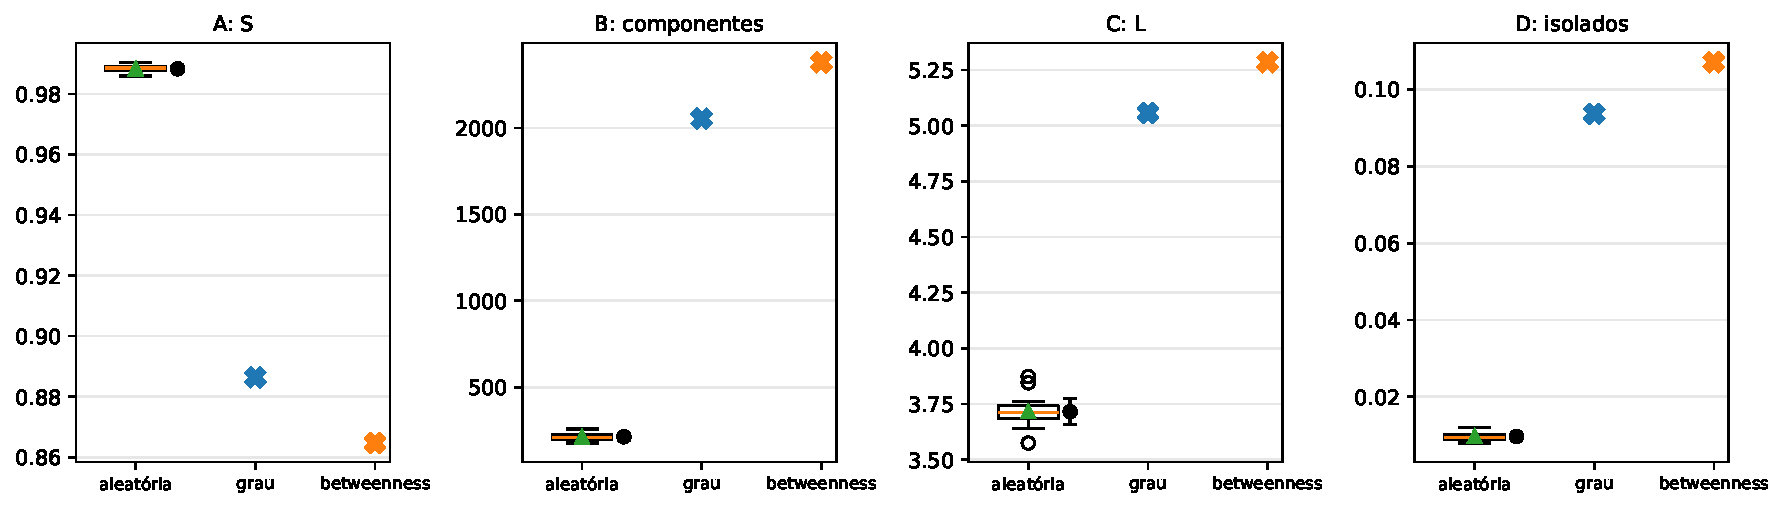
\includegraphics[width=.72\textwidth]{imagens/parte3_robustez_boxplot.pdf}
\caption{Distribuição das quatro métricas nas 30 remoções aleatórias de 5\% (caixas). O triângulo verde marca a média, e o ponto preto com barra, a média \(\pm\) desvio padrão. Os X marcam os ataques por grau e por intermediação (\emph{betweenness}). As métricas A e D aparecem como frações de 0 a 1; na Tabela~\ref{tab:robustez}, em porcentagem.}
\Description{Os ataques, marcados por X, reduzem a maior componente e aumentam as componentes, o caminho médio e os isolados em relação às caixas da remoção aleatória.}
\label{fig:robustez}
\end{figure*}
\figura{parte3_curvas_ataque}
  {Fração \(S(f)\) dos vértices restantes na maior componente, em função da fração removida \(f\).}
  {A curva aleatória cai pouco. As curvas de ataque dirigido caem mais e trocam de ordem acima de 20 por cento.}
  {fig:curvas}

A remoção aleatória mantém 98,8\% dos remanescentes na maior
componente e pouco altera os caminhos. Os ataques reduzem \(S\) para
88,6\% (grau) e 86,5\% (intermediação). É uma queda de 10 a 12
pontos, e não o colapso \(S_{\mathrm{rand}}\gg S_{\mathrm{cent}}\) que
o Apêndice C associa a redes muito vulneráveis. O contraste forte
está nas outras métricas: o ataque por intermediação cria 11 vezes
mais componentes, multiplica por 11 a fração de isolados e deixa \(L\)
42\% acima do da remoção aleatória (Tabela~\ref{tab:robustez} e
Figura~\ref{fig:robustez}).

As métricas B e D explicam a queda de \(S\). No ataque por
intermediação, 13,5\% dos remanescentes saem da maior componente, e
10,7 desses pontos (79\%) são vértices isolados. No ataque por grau,
são 9,4 de 11,4 pontos (82\%). O ataque desprende a periferia,
sobretudo folhas presas a um hub ou a uma ponte, e o núcleo continua
conexo, embora com caminhos mais longos. Concluímos que a LCC é
robusta a falhas aleatórias e sofre degradação moderada sob ataque
direcionado: perde a periferia, mas não a conectividade do núcleo.

A Figura~\ref{fig:curvas} estende os ataques até remover 30\%
da rede. Para a curva aleatória, usamos uma única ordem aleatória
e seus prefixos. O ataque por intermediação reduz mais \(S(f)\) até
20\% de remoção. O ataque por grau passa a reduzir mais a partir
de 22,5\%, o próximo ponto medido. O desempenho relativo dos
rankings, ambos calculados antes das remoções, depende da fração
retirada.

\subsection{Descoberta mais interessante: o mapa dos consoles}
\label{sec:consoles}

A descoberta mais interessante é que a rede reconstrói o mercado de
consoles sem nunca ter visto um rótulo. A plataforma e o tipo não
entram na construção do grafo, mas organizam as suas arestas. Os
números desta seção vêm do notebook \texttt{04\_consoles}.

\paragraph{Homofilia por família.}
Com o rótulo bruto de plataforma, 52,4\% das arestas ligam produtos
da mesma plataforma, contra 11,5\% esperados se as pontas se ligassem
ao acaso. Com a família de console normalizada, a fração sobe para
55,2\%, contra 9,7\% esperados (5,7 vezes), e a assortatividade passa
de 0,46 para 0,50 (0,59 com pesos). Nas 1\,000 permutações de rótulos,
a fração nunca passou de 11,6\% (\(p<0{,}001\)). A Tabela~\ref{tab:homofilia}
resume as três rotulações; nela, ``Rót.'' é o número de rótulos
distintos e ``Perm.'' é o maior valor entre as permutações.

\begin{table}[tbp]
\centering
\caption{Arestas com as duas pontas no mesmo rótulo: observado, esperado pela mistura ao acaso (\(\sum_a a_a^2\)), assortatividade \(r\) e máximo de 1\,000 permutações.}
\label{tab:homofilia}
\small
\setlength{\tabcolsep}{3.5pt}
\begin{tabular}{@{}lrrrrr@{}}
\toprule
Rótulo & Rót. & Obs. & Esp. & \(r\) & Perm. \\
\midrule
Plataforma bruta & 18 & 52,4\% & 11,5\% & 0,46 & 16,4\% \\
Família & 40 & 55,2\% & 9,7\% & 0,50 & 11,6\% \\
Classe & 6 & 63,0\% & 37,9\% & 0,40 & 36,0\% \\
\bottomrule
\end{tabular}
\end{table}

\paragraph{Os consoles concentram ligações.}
Os 290 consoles são 1,4\% dos produtos da LCC, mas têm 2,9\% das
pontas de aresta. O grau médio deles é 64, contra 30 na rede. A força é desigual também
entre eles: o Gini é 0,76, e os cinco mais fortes (PlayStation 4
500GB, Xbox One com Kinect, o pacote do Xbox 360 com Gears of War 3,
o Nintendo DS Lite e o pacote do Xbox One com Assassin's Creed Unity)
somam 24,5\% da força dos consoles. A categoria \emph{Consoles} da
Amazon inclui pacotes com jogo.

\paragraph{Hardware se liga a hardware.}
A matriz de mistura entre as classes mostra
que console--console ocorre 2,8 vezes mais que ao acaso e
acessório--acessório 2,7 vezes. Console--acessório fica em 1,2, e
console--jogo em 1,0, exatamente o acaso. Quem avalia um console
avalia outros aparelhos e periféricos, mas não mais jogos do que o
esperado. Os jogos retrô formam o grupo mais fechado (5,3 vezes), pois
pertencem a gerações que quase não se misturam com as atuais.


\paragraph{Rivalidade e troca de geração.}
Do peso das arestas console--console, 54\% fica na mesma família,
entre modelos e pacotes do mesmo aparelho. Os outros 46\% ligam
famílias diferentes, ou seja, usuários com mais de um console. Os
maiores pares cruzados são PlayStation 4 com Xbox One (134), os rivais
da mesma geração, e Xbox 360 com Xbox One (119), a troca de geração na
mesma marca. Em seguida vêm Nintendo DS com PSP (68), os portáteis
rivais.

\paragraph{As panelas, vistas de perto.}
A Figura~\ref{fig:panelas} reduz a rede a dois desenhos legíveis. À
esquerda, cada família com ao menos 100 produtos vira um vértice e se
liga às duas famílias com que mais se mistura acima do acaso. Das 30
ligações, 20 unem famílias do mesmo fabricante, e o desenho segue as
gerações: Wii, Wii U, 3DS e DS de um lado; PlayStation 3, 4 e Vita de
outro; Xbox, 360 e One em sequência; e os retrô, em que NES, Super
Nintendo e Mega Drive (Sega Genesis) se misturam até 25 vezes mais que
o acaso. À direita estão os 30 produtos mais fortes de cada uma das
12 maiores famílias, com só as três arestas mais pesadas de cada
produto. A redução não favorece a família, e mesmo assim 83\% das
arestas ficam dentro dela. Na rede inteira, a fração entre as três
arestas mais pesadas de cada produto é 76\%, contra 55\% em todas as
arestas: quanto mais forte a coavaliação, mais ela fica dentro da
família. As exceções formam a região central, em que PlayStation 2,
PSP e PC dividem o público.

\begin{figure*}[tbp]
\centering
\begin{minipage}[t]{.47\textwidth}
  \centering
  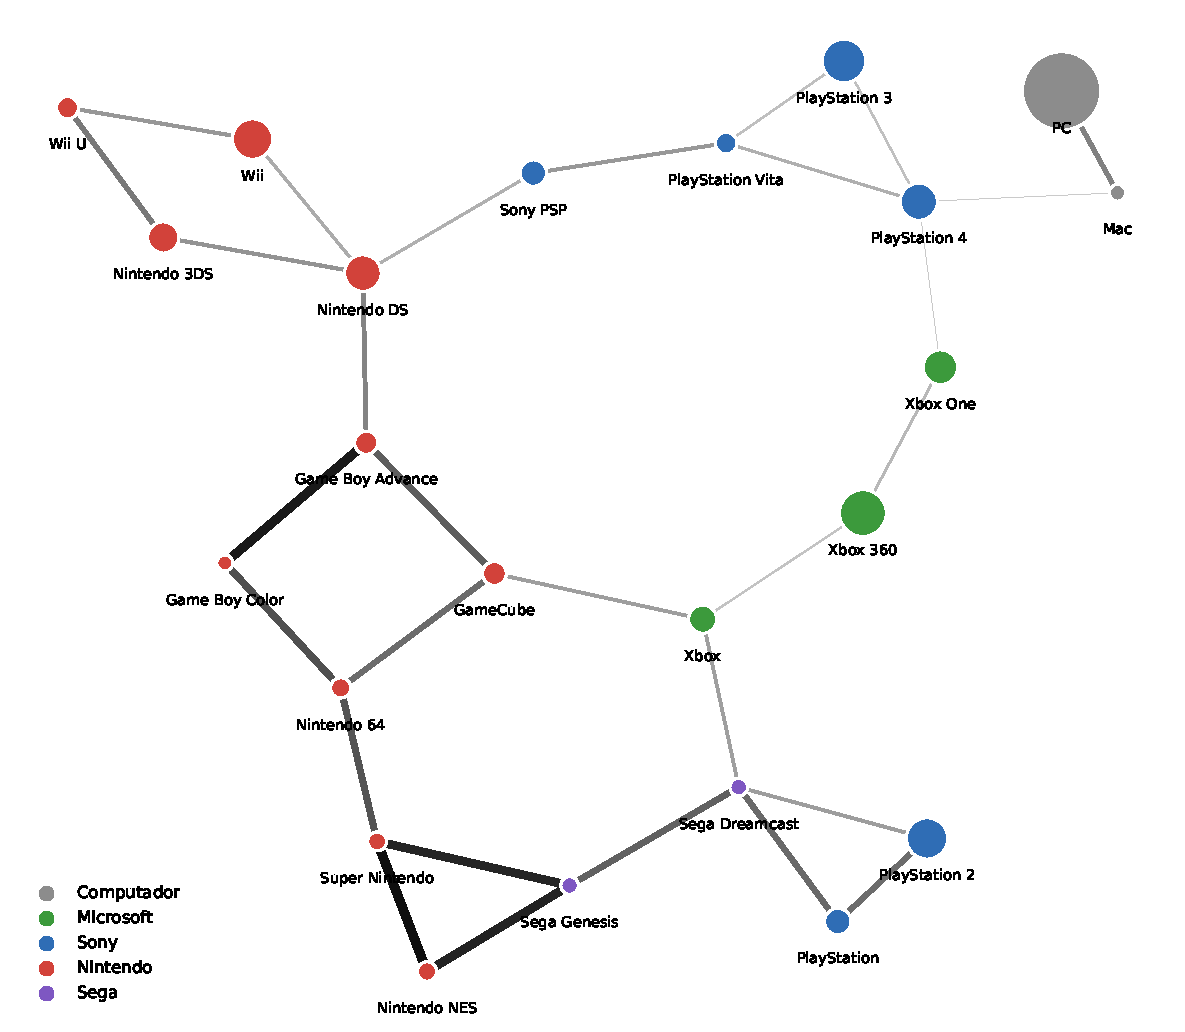
\includegraphics[width=\linewidth]{imagens/parte3_mapa_familias.pdf}
\end{minipage}\hfill
\begin{minipage}[t]{.51\textwidth}
  \centering
  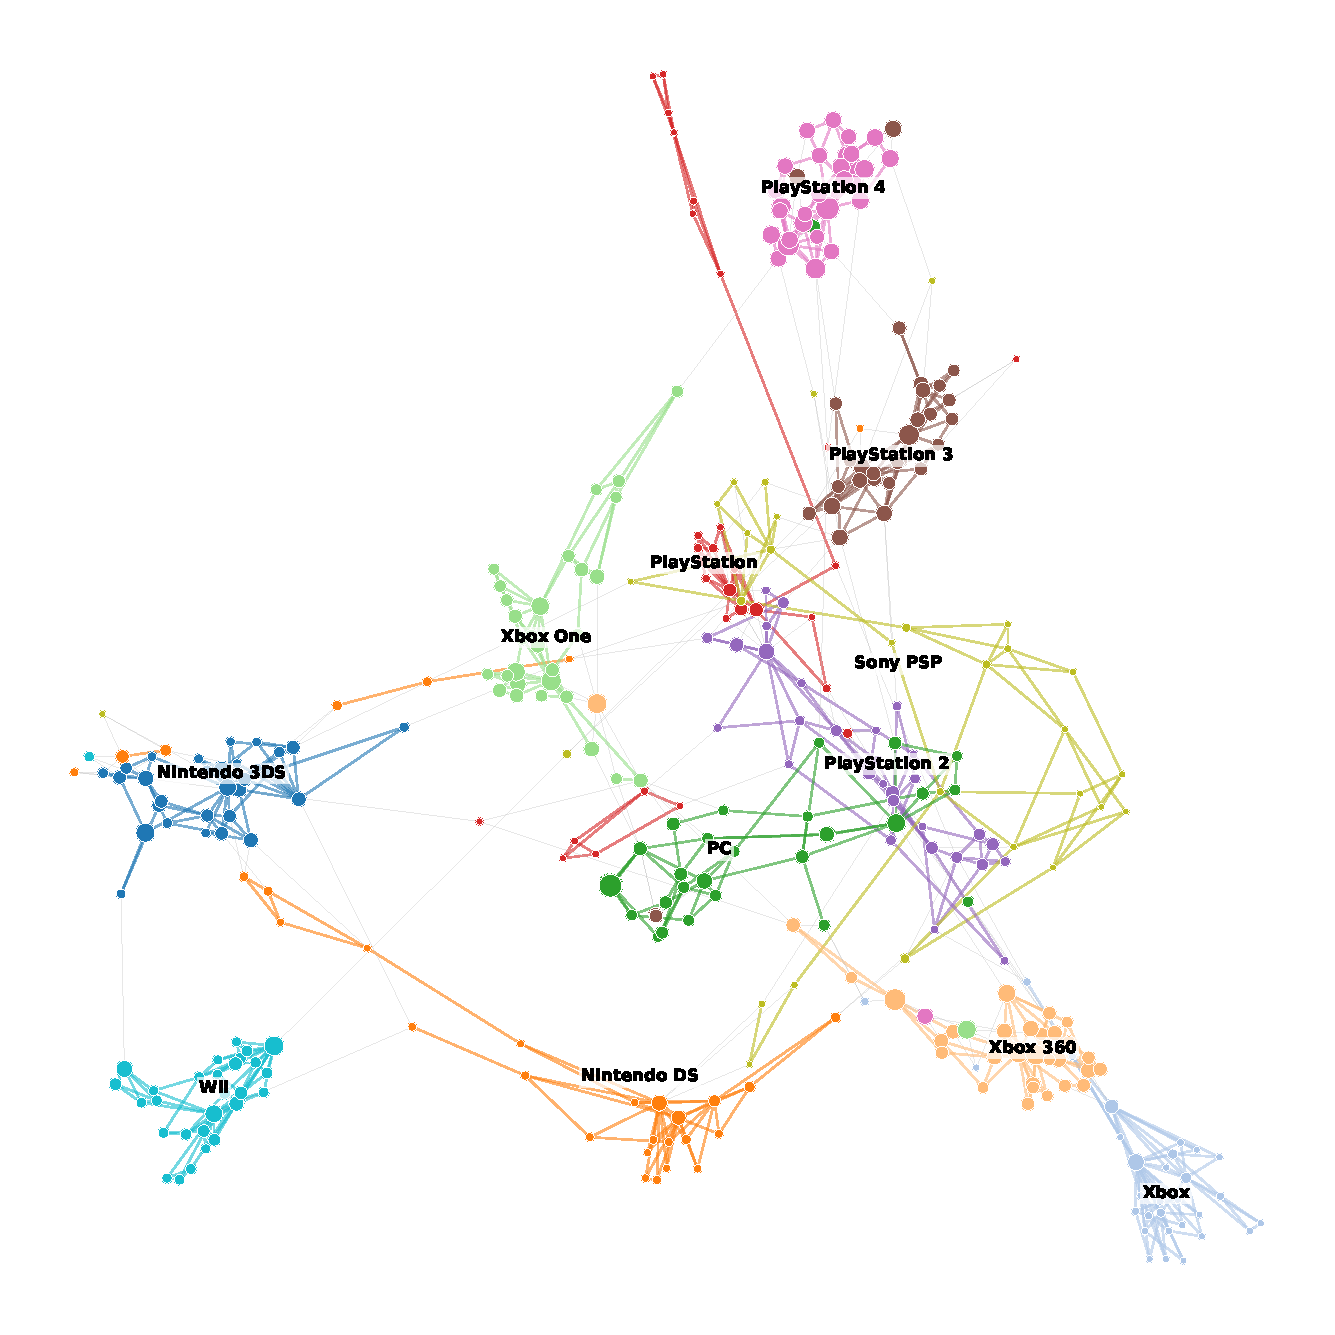
\includegraphics[width=\linewidth]{imagens/parte3_panelas.pdf}
\end{minipage}
\caption{Visualizações reduzidas das famílias de console. Esquerda: grafo entre famílias, com cor por fabricante, tamanho pelo catálogo e espessura pela razão entre a mistura observada e a esperada; cada família se liga às duas parceiras mais fortes. Direita: 30 produtos mais fortes de cada uma das 12 maiores famílias, com as três arestas mais pesadas de cada produto; arestas dentro da família na cor dela e entre famílias em cinza.}
\Description{À esquerda, as famílias formam cadeias por fabricante e geração, com os consoles retrô fortemente ligados. À direita, os produtos formam grupos compactos por família, como PlayStation 4, Wii, Xbox e Nintendo DS, com PlayStation 2, PSP e PC misturados no centro.}
\label{fig:panelas}
\end{figure*}

\paragraph{Os consoles não são os hubs.}
Nenhum console está entre os 20 maiores graus. Eles são 3,7\% dos \(r\)
vértices do topo por grau e 2,4\% por intermediação: mais que sua fração na rede,
mas pouco. O maior grau é do controle sem fio do Xbox 360 (1\,274
vizinhos), um acessório, que fica em quarto lugar em intermediação. A
maior ponte é o próprio Wii (1\,210 vizinhos), mas ele está sem tipo
nos metadados e cai em ``sem rótulo''; por isso a classe console é um
limite inferior. O jogo \emph{Big Kahuna Reef} é a segunda maior
ponte e fica fora dos 12 primeiros por grau: um título casual de PC
que liga o público de família ao resto do catálogo. Ter muitos
vizinhos e participar de muitos caminhos mínimos são papéis
diferentes.

\paragraph{O ataque solta ilhas de plataforma.}
Os grupos que se separam da maior componente nos ataques são quase
homogêneos: seis produtos de Xbox 360 no ataque por intermediação e
dez produtos retrô no ataque por grau. Remover as pontes desfaz os
elos entre as famílias, e os nichos se soltam.

\subsection{Comparação com modelos clássicos}

Geramos com código próprio três réplicas de cada modelo clássico com
o mesmo número de vértices e quase o mesmo número de arestas da LCC:
Erdős--Rényi \(G(n,m)\); Barabási--Albert com \(m_0=15\) arestas por
vértice novo, a razão \(m/n\) arredondada; e Watts--Strogatz com
\(k=30\), o grau médio arredondado para par, e \(p=0{,}1\). Medimos
neles as mesmas grandezas do grafo real (Tabela~\ref{tab:modelos} e
Figura~\ref{fig:modelos}).

\begin{table}[tbp]
\centering
\caption{Grafo real e modelos clássicos (média de 3 réplicas). \(L\) usa 100 origens; \(\hat\gamma\) é o MLE da cauda; o nulo bipartido vem da Tabela~\ref{tab:pequeno-mundo}.}
\label{tab:modelos}
\small
\setlength{\tabcolsep}{3pt}
\begin{tabular}{@{}lrrrrr@{}}
\toprule
Grafo & \(C\) & \(L\) & \(k_{\max}\) & Grau 1 & \(\hat\gamma\) \\
\midrule
Real & 0,325 & 3,78 & 1\,274 & 18,6\% & 2,11 \\
Erdős--Rényi & 0,001 & 3,24 & 55 & 0\% & -- \\
Barabási--Albert & 0,009 & 2,99 & 863 & 0\% & 2,93 \\
Watts--Strogatz & 0,530 & 4,09 & 38 & 0\% & -- \\
Nulo bipartido & 0,359 & 2,89 & -- & -- & -- \\
\bottomrule
\end{tabular}
\end{table}

\figura{parte3_modelos_ccdf}
  {Distribuição acumulada complementar dos graus do grafo real e de uma réplica de cada modelo clássico.}
  {A curva real decai lentamente até grau 1274; Barabási-Albert tem cauda mais curta; Erdős-Rényi e Watts-Strogatz caem abruptamente perto da média.}
  {fig:modelos}

Nenhum dos três modelos descreve a rede sozinho. Erdős--Rényi fica
230 vezes abaixo da clusterização observada e tem grau máximo 55, sem
cauda. Watts--Strogatz reproduz o agrupamento, até com sobra
(\(C=0{,}53\)), mas seus graus ficam perto da média (máximo 38) e seus
caminhos são mais longos que os reais. Barabási--Albert é o mais
próximo na distribuição de graus: gera hubs e uma lei de potência
quase perfeita (\(\hat\gamma=2{,}93\), perto do 3 teórico). Ainda
assim, sua clusterização é 38 vezes menor, ele não tem vértices de
grau 1, contra 18,6\% no grafo real, e sua cauda é mais leve. Nos
modelos sem cauda pesada, o ajuste de \(\hat\gamma\) não tem sentido e
foi omitido. O único que reproduz o agrupamento é o nulo bipartido
(0,359 contra 0,325), porque usa o mesmo mecanismo da rede: cada
usuário vira um clique. O grafo combina, portanto, a cauda pesada do
Barabási--Albert com um agrupamento que vem da projeção, e não de um
anel religado. O caminho médio real, mais longo que o do nulo, é o
que resta de estrutura própria: a segregação por família de console.

\section{Discussão crítica}

\paragraph{O modelo nulo decide a resposta.}
A pergunta ``a rede é pequeno mundo?'' teve duas respostas opostas,
conforme a referência. Contra Erdős--Rényi, \(\sigma=196\); contra o
nulo bipartido, \(\sigma=0{,}69\). A segunda é a mais informativa:
qualquer projeção de um bipartido gera cliques, então o \(C\) alto é
efeito do método, não um mecanismo da rede. O erro simétrico também é
possível. Se a análise fosse feita no próprio bipartido
usuário--produto, sem projeção, \(C\) seria zero por construção, pois
um grafo bipartido não tem ciclos ímpares nem triângulos, e
\(\sigma\) seria 0 por outro artefato. O que o nulo bipartido revela é
outra coisa: a rede real tem \(L\) maior que o dele (3,78 contra
2,89). Os caminhos são mais longos do que coavaliações ao acaso
produziriam, e a homofilia por família da Seção~\ref{sec:consoles}
explica por quê: os produtos ficam presos à sua família de console.
O mesmo cuidado vale para a homofilia, cuja referência analítica
(11,5\%, plataforma bruta) e cuja permutação de rótulos (média de
15,3\% e máximo de 16,4\%, mesmo rótulo) diferem porque
preservam coisas diferentes. Nos dois casos, o observado fica muito
acima. A comparação com o nulo bipartido tem limites: são só três
réplicas, e a maior componente delas tem cerca de 14 mil vértices,
contra 21 mil na rede real.

\paragraph{Avaliar não é comprar.}
Uma aresta registra que dois produtos têm avaliadores em comum. O
CSV de 2018 não informa se a compra foi verificada, e quem avalia é
uma fração dos compradores, enviesada para quem escreve muito. Por
isso, a ``concentração de compra de consoles'' da Seção~\ref{sec:consoles} é uma
concentração de \emph{coavaliações}. Filtrar avaliações de compra
verificada, campo que existe nos arquivos completos da coleção,
aproximaria melhor a compra conjunta.

\paragraph{O tratamento define a rede.}
Os 456 usuários com mais de 50 produtos eram 0,03\% dos avaliadores,
mas geravam 47,5\% das ocorrências de pares. Sem o corte T2, a
projeção refletiria poucos colecionadores. A poda T5 decide quanto da
rede sobra: com peso mínimo 1, 2 ou 3, a maior componente tem 98,8\%,
58,1\% ou 33,2\% dos produtos (Tabela~\ref{tab:limiar}). Esperamos
que a cauda pesada, a sensibilidade a ataques e a homofilia resistam a
esses cortes, porque dependem de diferenças de ordens de grandeza.
Já \(C\), \(L\) e o número de componentes dependem diretamente do
limiar. Ainda não repetimos as Partes I e III em outros limiares, e
essa é a principal verificação pendente. A projeção também apaga o
usuário: um par avaliado por alguém que avaliou dois produtos pesa o
mesmo que um par avaliado por alguém que avaliou cinquenta. Ponderar
cada contribuição por \(1/(k_u-1)\) reduziria o peso dos perfis
amplos.

\paragraph{O tempo foi apagado.}
A rede une avaliações de 1997 a 2018. Uma aresta pode ligar produtos
avaliados com anos de diferença, e isso muda a leitura dos pares de consoles: o par
Xbox 360--Xbox One pode ser troca de geração, e o par PlayStation
4--Xbox One, posse simultânea de rivais. Só uma análise por janelas
de tempo separaria as duas leituras.

\paragraph{Fonte e rótulos.}
A troca para a edição de 2018 (Seção~\ref{sec:determinacao}) impede comparar os tamanhos
com os da planilha da disciplina. Os rótulos vêm de
\emph{scraping}: 728 produtos da LCC têm restos de HTML no tipo, o
próprio Wii está sem tipo, e a categoria \emph{Consoles} inclui
pacotes com jogo. As frações por classe são, portanto, limites
inferiores, e a homofilia se refere aos rótulos disponíveis.

\paragraph{Pontes e hubs.}
O ataque por intermediação é mais destrutivo até 20\% de remoção, e o
ataque por grau passa a ser a partir de 22,5\%
(Figura~\ref{fig:curvas}). A análise dos consoles sugere a razão: a intermediação
remove primeiro as pontes entre famílias, como o Wii, o DS Lite e
\emph{Big Kahuna Reef}, e isola as famílias. Depois disso, o que
fragmenta cada família são os seus hubs internos, que o ranking por
grau alcança. Os dois rankings são fixos. Um ataque adaptativo, que
recalcula a centralidade após cada remoção, tende a ser mais
destrutivo e não foi medido.

\paragraph{Tempos e lei de potência.}
A bola de neve parte do maior hub, então os subgrafos pequenos são
mais densos que a rede: \(m/n\) fica entre 30 e 38 nos subgrafos de
1\,000 a 8\,000 vértices e cai para 15 na LCC. Isso entra nas
inclinações de 1,01 a 1,16 dos algoritmos lineares, porque uma única
constante para \(n+m\) supõe que vértice e aresta custam o mesmo. O
Bellman--Ford para quando uma rodada não altera nenhuma distância;
num grafo de diâmetro 13, isso ocorre depois de poucas rodadas
\(k\), e o custo efetivo \(O(k\,m)\) explica a inclinação de 0,65
contra \(nm\). O
Floyd--Warshall só foi medido até 800 vértices. Na lei de potência, a
lognormal ganhou da lei pura. Isso é coerente com a projeção, porque o
grau de um produto acumula as vizinhanças de seus avaliadores, um
processo mais próximo de multiplicativo que de ligação preferencial.

\section{Conclusão}

A rede de coavaliações tem poucos pares ligados diretamente, mas
caminhos curtos dentro da maior componente. A cauda dos graus é
pesada, sem ser uma lei de potência pura. A rede resiste a falhas
aleatórias, e os ataques direcionados a degradam só moderadamente:
soltam a periferia, mas o núcleo continua conexo. O agrupamento elevado vem da projeção em cliques, como
mostrou o nulo bipartido, e não deve ser lido como propriedade da
rede. O achado mais forte é a organização por família de console:
55,2\% das arestas ficam dentro da família, contra 9,7\% ao acaso,
e os consoles concentram ligações com outros aparelhos, inclusive de
marcas rivais. Entre os modelos clássicos, nenhum reproduz a rede:
Barabási--Albert acerta a cauda, e só a projeção de um bipartido
aleatório acerta o agrupamento.

Como próximos passos, propomos repetir as medidas nos limiares
alternativos, filtrar compras verificadas, separar janelas de tempo
para distinguir rivalidade de troca de geração e ampliar as réplicas
do nulo bipartido, controlando o tamanho da componente.

\begin{thebibliography}{9}
\bibitem{snapamazon} Stanford Network Analysis Project.
\emph{Web data: Amazon reviews}.
\url{https://snap.stanford.edu/data/web-Amazon.html}.

\bibitem{acessosnap} Stanford Network Analysis Project.
\emph{Aviso de acesso à coleção de avaliações da Amazon}.
\url{https://snap.stanford.edu/data/amazon/amazon_readme.txt}.

\bibitem{amazon2018} Jianmo Ni. 2018.
\emph{Amazon Review Data (2018)}. University of California San Diego.
\url{https://cseweb.ucsd.edu/~jmcauley/datasets/amazon_v2/}.

\bibitem{ni2019} Jianmo Ni, Jiacheng Li e Julian McAuley. 2019.
Justifying Recommendations using Distantly-Labeled Reviews and Fine-Grained Aspects.
Em \emph{EMNLP-IJCNLP}, 188--197.
\url{https://doi.org/10.18653/v1/D19-1018}.

\bibitem{watts1998} Duncan J. Watts e Steven H. Strogatz. 1998.
Collective dynamics of 'small-world' networks.
\emph{Nature} 393, 440--442.
\url{https://doi.org/10.1038/30918}.

\bibitem{newman2001} M. E. J. Newman, Steven H. Strogatz e Duncan J. Watts. 2001.
Random graphs with arbitrary degree distributions and their applications.
\emph{Physical Review E} 64, 026118.
\url{https://doi.org/10.1103/PhysRevE.64.026118}.

\bibitem{humphries2008} Mark D. Humphries e Kevin Gurney. 2008.
Network 'Small-World-Ness': A Quantitative Method for Determining Canonical Network Equivalence.
\emph{PLoS ONE} 3(4), e0002051.
\url{https://doi.org/10.1371/journal.pone.0002051}.

\bibitem{newman2003} M. E. J. Newman. 2003.
Mixing patterns in networks.
\emph{Physical Review E} 67, 026126.
\url{https://doi.org/10.1103/PhysRevE.67.026126}.

\bibitem{clauset2009} Aaron Clauset, Cosma Rohilla Shalizi e M. E. J. Newman. 2009.
Power-Law Distributions in Empirical Data.
\emph{SIAM Review} 51(4), 661--703.
\url{https://doi.org/10.1137/070710111}.
\end{thebibliography}

\end{document}
